% XeLaTeX; manuscript source, not compiled in this delivery.
\documentclass[UTF8,fontset=fandol,11pt,a4paper]{ctexart}
\usepackage[margin=2.4cm]{geometry}
\usepackage{amsmath,amssymb,booktabs,graphicx,hyperref}
\graphicspath{{figures/}}
\title{全域干燥终点的数值验证与模型结构敏感性\\\large 基于107个已完成情景的论文素材}
\author{}
\date{2026年9月12日}
\begin{document}
\maketitle
\noindent\textbf{口径提示：本稿属于经验热容量闭合、不计显式汽化热的对照实验，不替代仓库守恒显热或相变工况结论。}

\begin{abstract}
为避免平均含水率掩盖内部湿区，本文以全域最大干基含水率首次达到阈值定义干燥终点，并采用材料坐标下的径向模型开展结构与系数对照。107个情景表明，基准Q3和Q4的全域达标时间分别为57.47 h和51.09 h；在45组匹配扩散扰动中，Q4均提前5.49--7.39 h。然而，相同外半径观测下改变内部变形映射或表面传质通量的密度定义，部分情景发生排序反转。结果表明，基准优势不能脱离物理闭合条件推广。
\end{abstract}
\section{终点定义}
令$C(a,t)$为干基含水率，$a\in[0,1]$为材料径向坐标，$C_*=0.15$。定义
\begin{align}
 t_{\max}&=\inf\{t:\max_{a\in[0,1]}C(a,t)\le C_*\},\\
 t_{\mathrm{mean}}&=\inf\{t:\bar C(t)\le C_*\},\qquad
 \bar C(t)=\frac{\int C\,\mathrm d m_d}{\int\mathrm d m_d},\\
 t_{\mathrm{tail}}&=t_{\max}-t_{\mathrm{mean}}.
\end{align}
数值实现以节点最大值近似连续空间最大值，其精度仍需网格检验。首次达标不自动证明所有后续时刻均达标。配对差定义为候选减参照，负值表示加快。
\section{基准与几何控制}
\begin{table}[htbp]\centering
\caption{达标时间，单位：h。}
\begin{tabular}{lrrr}\toprule
工况 & 平均达标 & 全域达标 & 间隔\\\midrule
Q3固定半径基准 &36.02&57.47&21.45\\
Q4观测收缩仿射基准 &34.97&51.09&16.12\\
Q3施加观测收缩 &17.42&25.24&7.82\\
Q4固定半径控制 &85.03&129.85&44.82\\\bottomrule
\end{tabular}\end{table}
平均达标不能代替全域达标。基准Q4提前6.39 h（11.11\%），但Q3/Q4同时改变物性和几何，不能将全部差异归因于收缩。同一Q4物性下，观测收缩使终点由129.85 h降至51.09 h；几何还影响密度和边界通量，不能仅解释为距离缩短。固定Q4允许积分至168 h，未外推观测收缩曲线。
\section{内部变形与边界定义}
\begin{figure}[htbp]\centering
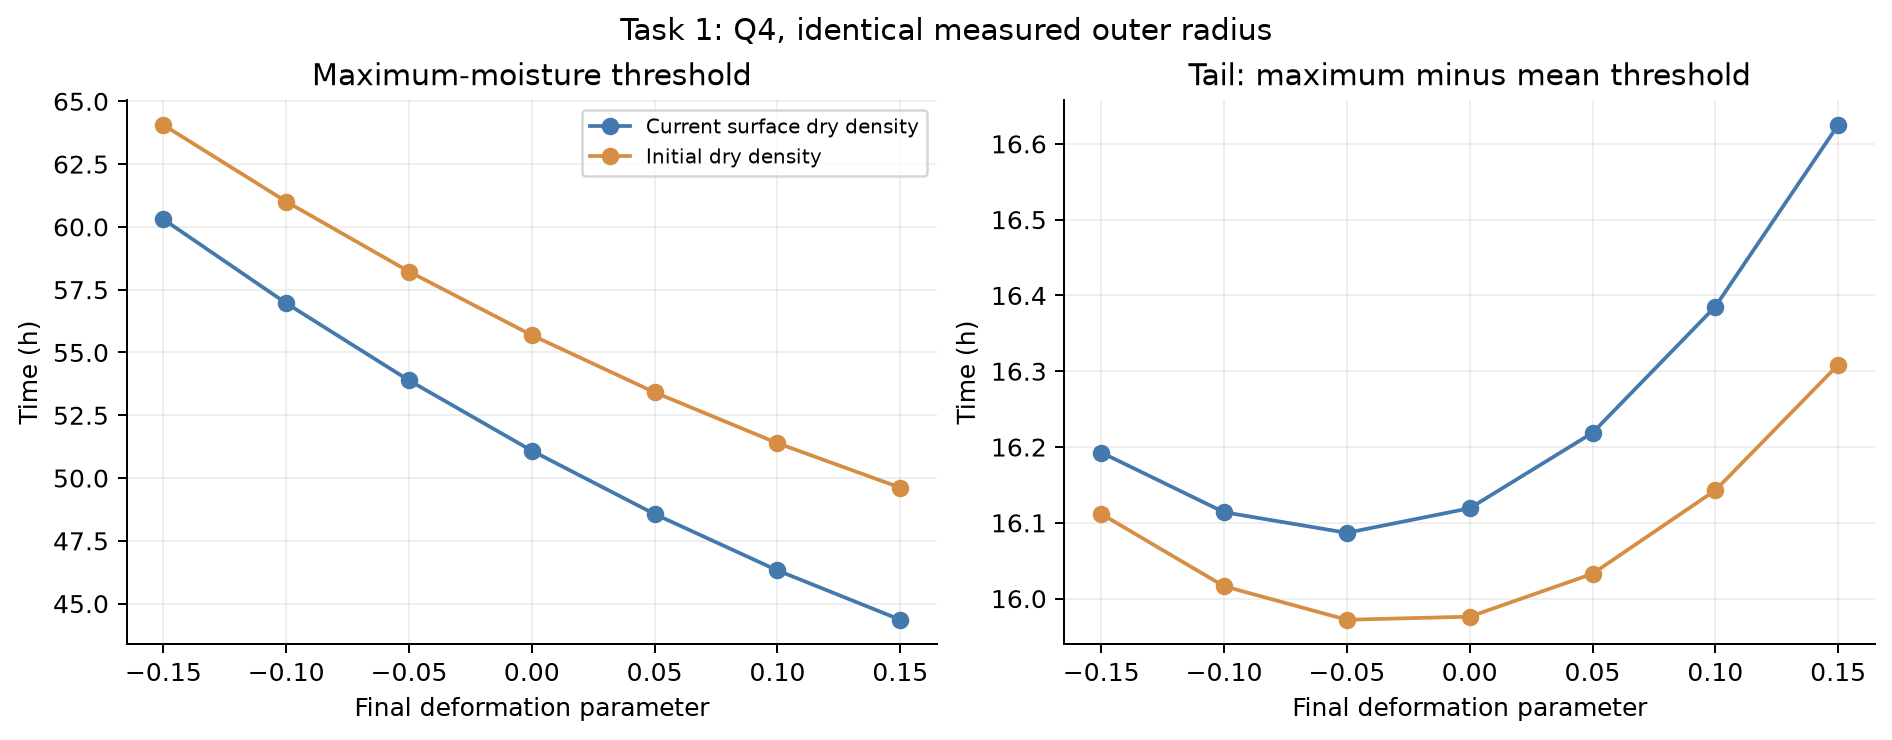
\includegraphics[width=\linewidth]{analysis_task1_deformation.png}
\caption{同一外半径下，变形与边界密度定义的影响。左为全域终点，右为尾段。蓝色使用当前表面干密度，橙色使用初始干密度。连线仅辅助阅读；纵轴未从零开始。}
\end{figure}
当前干密度边界下，最终变形参数由$-0.15$至$+0.15$时，终点由60.30 h降至44.36 h，相对仿射基准变化约$+18.04\%$至$-13.17\%$。部分情景超过Q3基准的57.47 h。因此外半径观测不足以在本模型族中唯一决定内部干燥过程。

仿射基准改用初始干密度边界后，终点由51.09 h增至55.69 h，增加4.60 h。尾段约15.97--16.62 h且并非单调下降，更早全域达标不必然意味着更短尾段。
\section{区域扩散扰动}
扰动为$D_{\mathrm{new}}=D_{\mathrm{base}}\exp(\delta m)$，$m$为平滑窗口。$\delta=0.10$在$m=1$处约增加10.52\%。
\begin{figure}[htbp]\centering
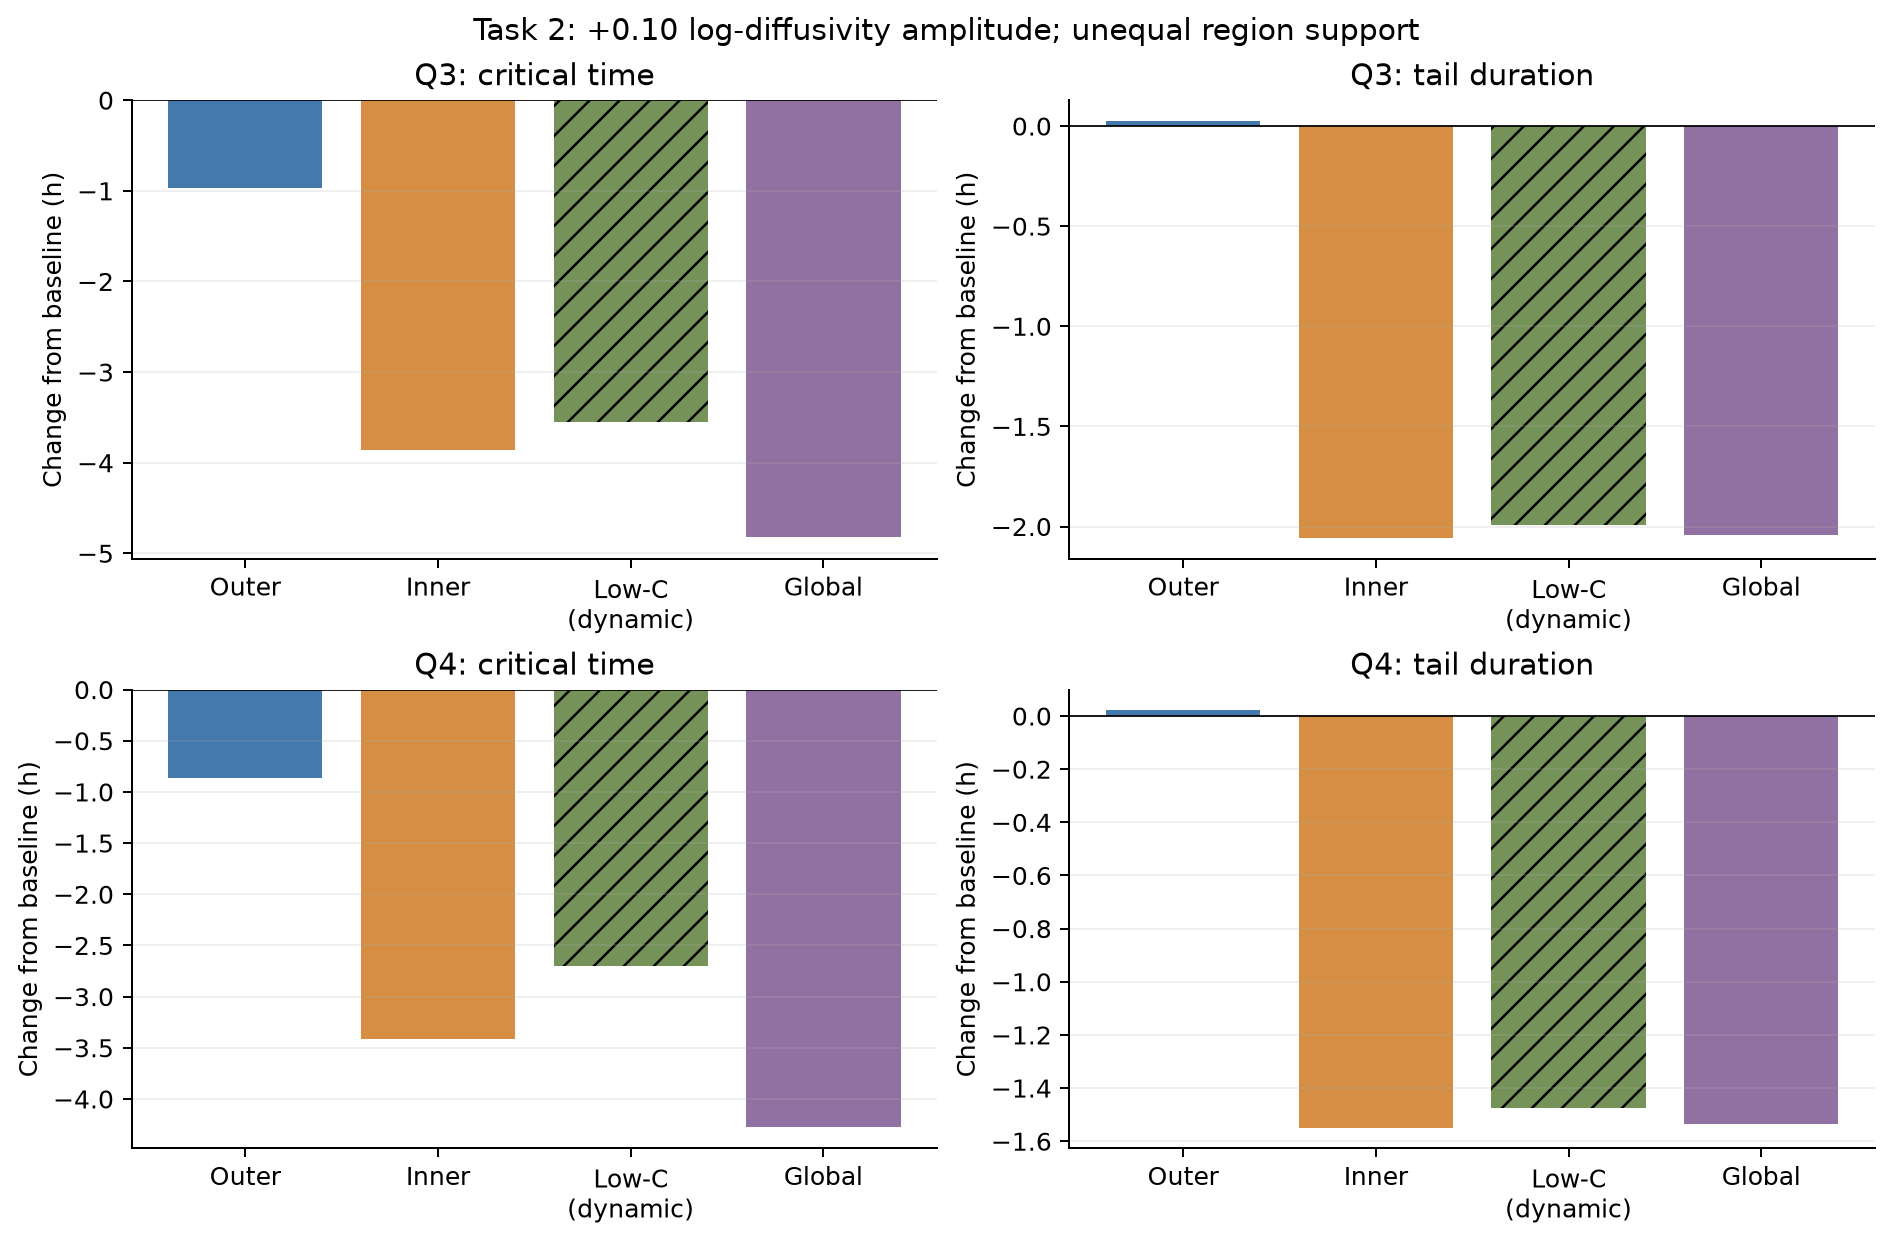
\includegraphics[width=.95\linewidth]{analysis_task2_effects.png}
\caption{正向对数扩散扰动0.10下的终点与尾段变化。内外层材料坐标宽度0.10，低含水率阈值0.20、平滑宽度0.02。负值表示缩短；不同区域作用范围不等。}
\label{fig:effects}\end{figure}
Q4外层、内层、低含水率及全域扰动分别缩短终点0.86、3.41、2.70、4.27 h。内外层分别覆盖约81.01\%与18.99\%，故总效应不等于局部敏感性。
\begin{figure}[htbp]\centering
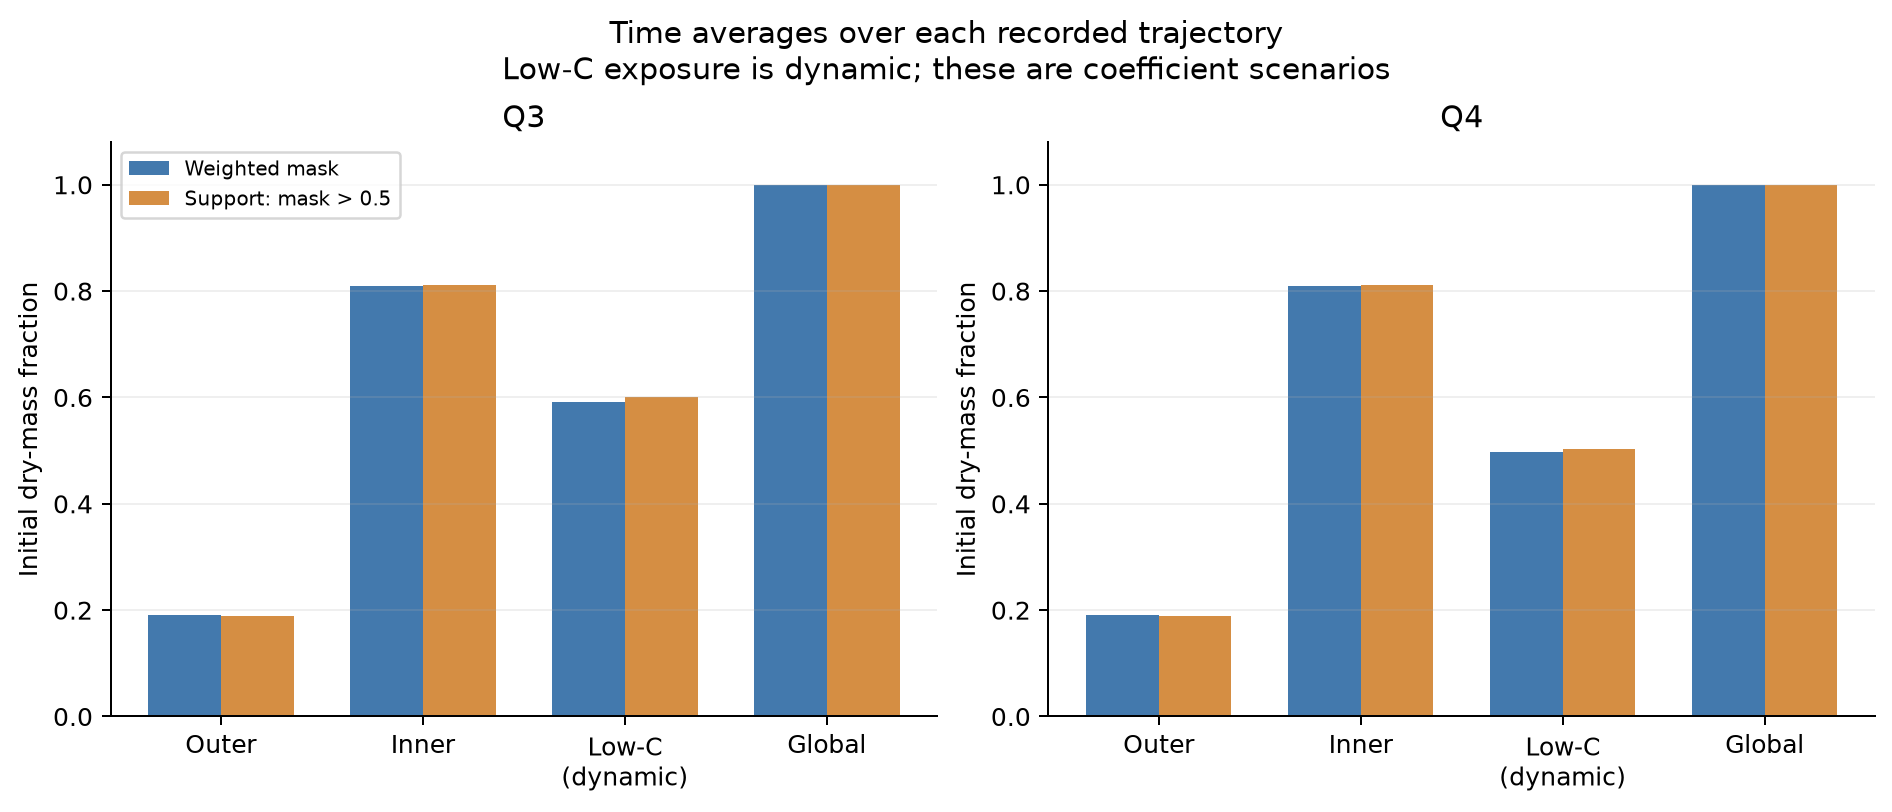
\includegraphics[width=\linewidth]{analysis_task2_exposure.png}
\caption{图\ref{fig:effects}各扰动沿自身轨迹的平均作用范围。蓝色为平滑窗口质量加权均值，橙色为窗口超过0.5的干物质占比。低含水率窗口受状态影响，不能视为等价的外生固定剂量。}
\end{figure}
静态区域可用描述性中心差分
\begin{equation}
 S_m=\frac{t_{\max}(+\delta)-t_{\max}(-\delta)}{2\delta\bar m}
\end{equation}
衡量单位质量加权范围的变化。幅度0.10、宽度0.10下，外层与内层$|S_m|$比值在Q3、Q4中约为1.063、1.075。外层略高但无压倒性优势；有限扰动差分不等于无穷小导数，也不是严格等剂量优化试验。
\section{交叉证据}
按扰动类型、幅度、宽度、阈值及平滑宽度逐项匹配，共45组Q3/Q4，均保持Q4更快，领先5.494--7.386 h。结合结构试验，本轮支持：\textbf{基准排序对所测试扩散扰动保持稳定，但会随内部变形与边界定义改变。}设计点不是独立随机样本，45/45不能解释为概率100\%。
\section{验证与局限}
单张H100、FP64的15项CUDA验收全部通过，四个全时域代表工况的同网格CPU/GPU终点差为0.158--0.241 s。这不是107个情景的统一空间误差上界，也不是实验验证。

独立采样通量积分残差绝对值最大约0.0352\%，包含采样误差。经验湿密度与几何反算的干质量除以守恒干质量，在Q4收缩基准约为0.890；这是闭合兼容性诊断，不能称为实际干物质损失11\%。

验收6.19 min，主计算47.76 min；无公平CPU总耗时对照，不报告加速倍数。后续任务3应检验长期边界与物性结构的联合影响，并在排序翻转附近针对性加密，不应提前写入尚未得到的结论。
\appendix
\section{来源与使用}
数据来自运行\texttt{20260912\_033943\_gpu}，107个情景全部完成。三图为服务器原始PNG。配对表、验证与环境记录随素材包提供。此次未重新运行模型，本文为可整合LaTeX稿，未编译PDF。更完整的写作建议和数字见随附Markdown；未补造实验结果或文献。
\end{document}
